\section{Commissioning Background Estimation Methods with 7TeV Data}

Having shown that the two background estimation methods work well in Monte Carlo simulation, we next take a look at the results using collision data, and, for comparison a Monte Carlo sample generated by PYTHIA8 to be non process-specific. 

It is intentional for this analysis to commission low-$p_{T}$ electrons (of offline thresholds below the standard online threshold of the single electron trigger); and therefore the data sample is chosen from the JetMETTau secondary datasets, which are subject to JetMET triggers. The data sample used in this study is taken from the Secondary Dataset (SD) JetMETTau, and the HLT trigger applied on top of the selection is the HLT\_Jet15U.

The 7TeV collision data used to demostrate the performance of the Background Estimation methods described in this Note, amounts to 12.47 $\text{nb}^{-1}$ of integrated luminosity.

\subsection{Commissioning the Isolation Template method with first data}

The data are selected as described in section~\ref{sec:evtsel}. Events with at least one electron with $p_{T}>$ 10 GeV and passing all standard electron identification, as well with a minimal hadronic activity of $H_{T} >$ 20 GeV - equivalent to the requirement of at least one jet with $p_{T}>$ 20 GeV -, are used to plot the combined Isolation distribution in the Selection region. A three-template fit is used to model the Isolation distribution in the Selection region, with two-template background component taken from the two control regions which defined earlier, and a single W-component to describe the $W \rightarrow e\nu$ shape. The W-shape is used here directly from a MC template ($We\nu$ PYTHIA sample) in order to test the Isolation template method.  

Figures~\ref{fig:d_combIso_fit} show the full fit to the Isolation distribution in the Selection region, with the right plot repeating the exercise with a $pfMET < 20$~GeV cut. In both cases there is a good agreement between the Isolation shape selected and the modeling distributions extracted from the control regions. A first evidence of W-signal contamination is apparent on the plots; with the left one showing an excess of events from the predicted background, and the right one showing the suppression of the signal using the pfMET ``anti-cut''. 

Since, as was shown in section~\ref{sec:modeling}, we observed a small deviation between the Calorimeter Isolation distributions in the Control and Selection Regions (prior to re-weighting as described above) we would like to confirm that the good description of the full Isolation distribution, i.e. with all backgrounds combined, remains good for different regions in the overall hadronic selection of the events.  For this reason, we repeat the fits for different values of the total $\text{H}_{T}$ of the event.  The fits yield a number of expected events passing the RelIso$<0.3$ requirement -- and this number can be compared to the actual number seen in the data.  We summarize these results in Figure~\ref{fig:d_fitprediction} where a very good agreement between the predicted and observed event yields is seen.


\begin{figure}[h!]
\centering
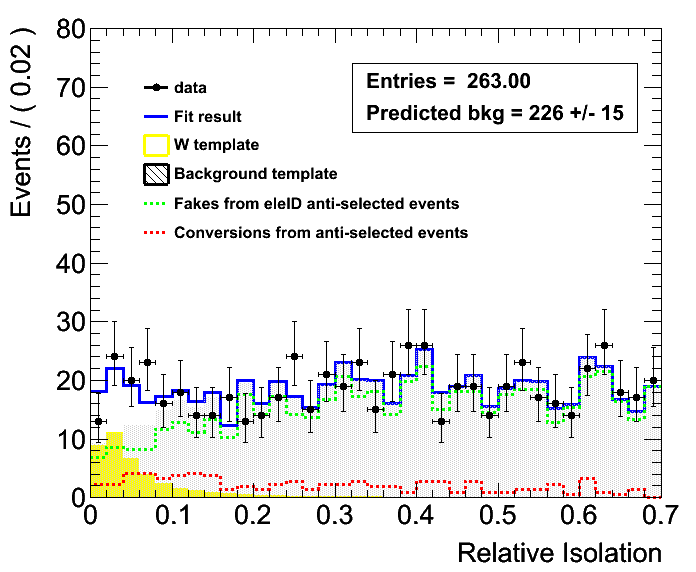
\includegraphics[scale=0.32]{Plots/d_combIso_pt10_fit.png}
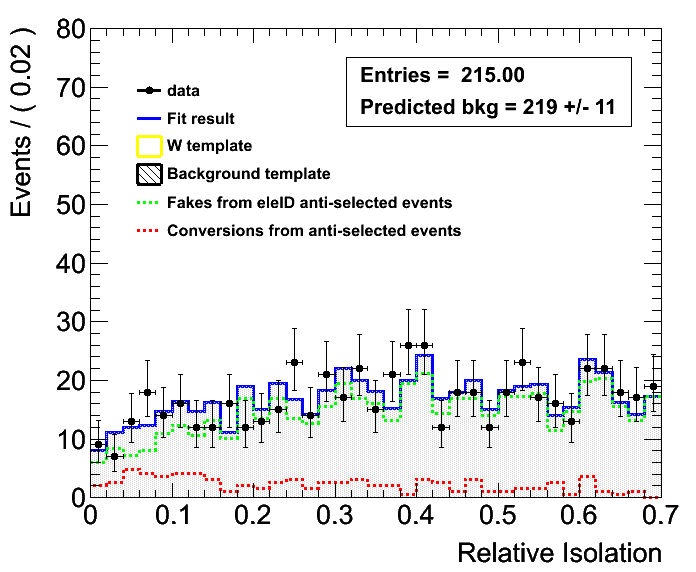
\includegraphics[scale=0.32]{Plots/d_combIso_pt10_METanticut_fit.png}
\caption{\textit{The combined Isolation distribution for 10 GeV electrons in data (points) and its breakdown into three components, one for the combined background from jets and heavy-flavors (Jet-e and HF-e), another for conversions (Conv-e) and a third for the W $\rightarrow e\nu$. The dashed lines are the two background components as extracted from the two Control Samples, whereas the sum of the ``predicted'' background is shown in filled grey. On the right plot, a pfMET $ < 20$~GeV anti-cut has been applied.  }}
\label{fig:d_combIso_fit}
\end{figure}

\begin{figure}[h!]
\centering
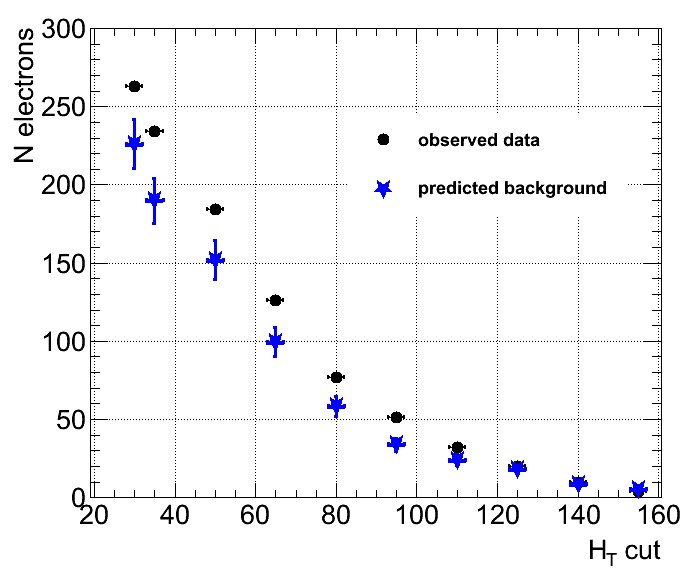
\includegraphics[scale=0.32]{Plots/d_fitprediction_pt10_vsHT.png}
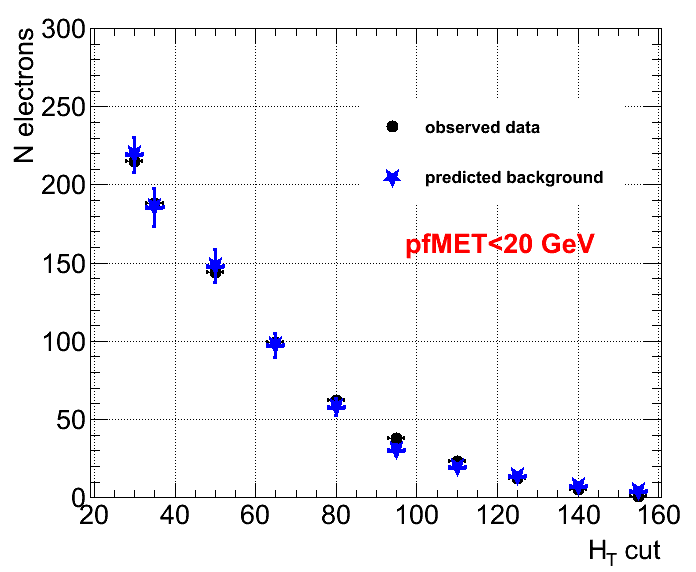
\includegraphics[scale=0.32]{Plots/d_fitprediction_pt10_METanticut_vsHT.png}
%\end{center}
\caption{\textit{The observed number of electrons (in black dots) in signal region, RelIso $< 0.3$, are compared to the fit prediction (in blue stars), as a function of the cut in the hadronic activity of the event ($H_{T}$ cut). A pfMET anti-cut at 20~GeV has been applied to suppress sources of prompt electrons (e.g. Ws). }}
\label{fig:d_fitprediction}
\end{figure}

%The same procedure is applied to events with electrons with $p_{T} >$ 20 GeV, and the result can be in inspected similarly on Figures~\ref{fig:d_combIso_fit_pt20} and~\ref{fig:d_fitprediction_pt20}. The evidence of the W component present in the selection is now more prominent with the level of background being significantly lower with respect to the $p_{T}(e)>10 $ GeV case. The overall results show a compatible behavior with the corresponding MC results presented in section~\ref{mc_wcontamin}. 


\begin{figure}[h!]
\centering
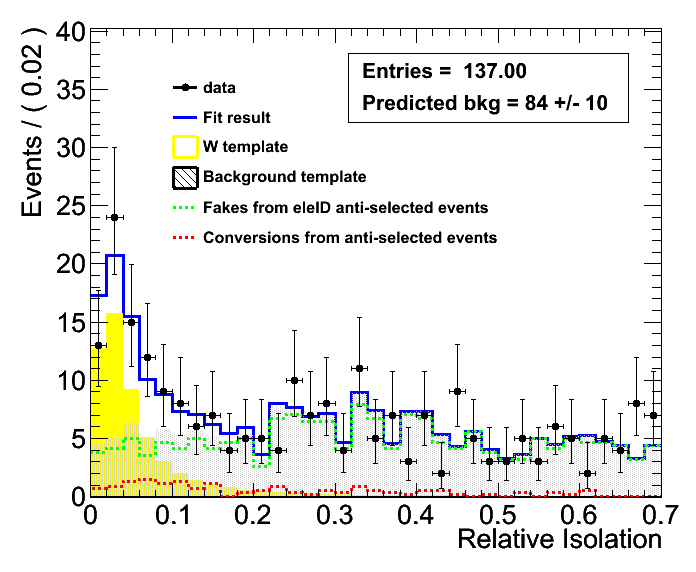
\includegraphics[scale=0.32]{Plots/d_combIso_pt20_fit.png}
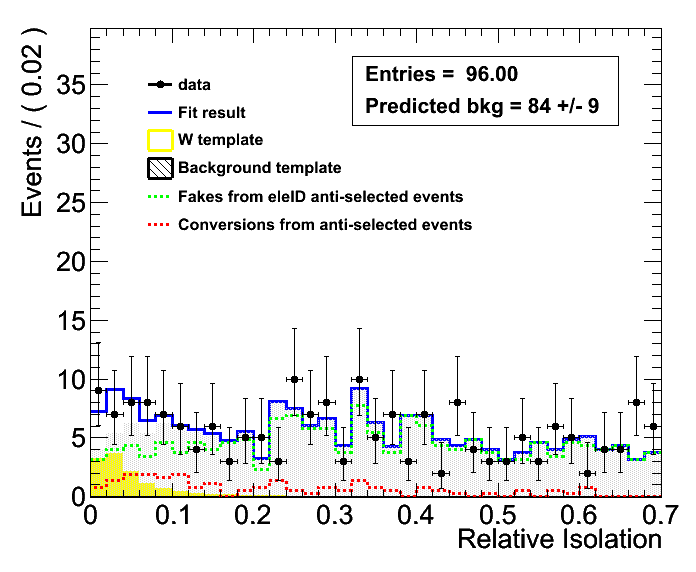
\includegraphics[scale=0.32]{Plots/d_combIso_pt20_METanticut_fit.png}
\caption{\textit{Same as Figure~\ref{fig:d_combIso_fit} only this time for electrons with $P_{T}$ threshold at 20 GeV.  }}
\label{fig:d_combIso_fit_pt20}
\end{figure}

\begin{figure}[h!]
\centering
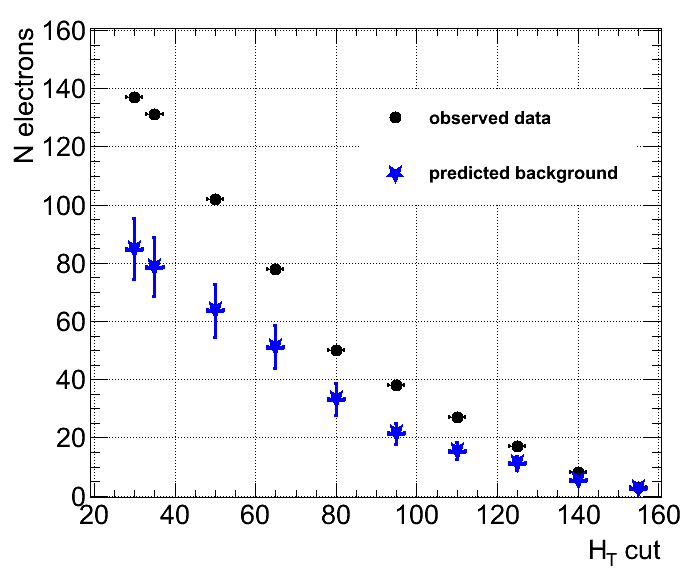
\includegraphics[scale=0.32]{Plots/d_fitprediction_pt20_vsHT.png}
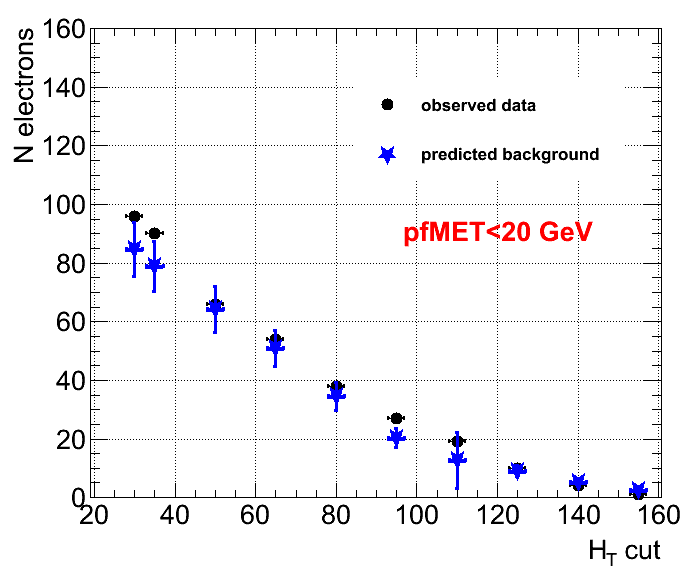
\includegraphics[scale=0.32]{Plots/d_fitprediction_pt20_METanticut_vsHT.png}
%\end{center}
\caption{\textit{Same as Figure~\ref{fig:d_fitprediction} only this time for electrons with $P_{T}$ threshold at 20 GeV. }}
\label{fig:d_fitprediction_pt20}
\end{figure}

The same procedure is applied to events with electrons with $p_{T} >$ 20 GeV, and the result can be in inspected similarly on Figures~\ref{fig:d_combIso_fit_pt20} and~\ref{fig:d_fitprediction_pt20}. The evidence of the W component present in the selection is now more prominent with the level of background being significantly lower with respect to the $p_{T}(e)>10 $ GeV case. The overall results show a compatible behavior with the corresponding MC results presented in section~\ref{mc_wcontamin}.

%The fits also yield a number of expected events passing the RelIso$<0.3$ requirement -- and this number can be compared to the actual number seen in the data.  We summarize these results in Table~\ref{tab:IsoFits} where a very good agreement between the predicted and observed event yields is seen.  

\begin{comment}
\begin{table}[h!]
\vspace{5mm}
\begin{center}
\begin{tabular}{|c||c|c||c|c|}
\hline
&\multicolumn{2}{c|}{$p_{T}(e) > 5 \text{GeV}$}&\multicolumn{2}{c|}{$p_{T}(e) > 10 \text{GeV}$}\\
\cline{2-5}
& \textbf{Observed} & \textbf{Predicted} & \textbf{Observed} &  \textbf{Predicted} \\
\hline
\hline
$H_{T}>20 \text{GeV}$ & $115.$ & $115.4 \pm 7.5$ & $98.$ & $99.6 \pm 7.4$ \\
$H_{T}>40 \text{GeV}$ & $54.$ & $56.5 \pm 5.3$ & $46.$ & $48.9 \pm 5.0$ \\
$H_{T}>60 \text{GeV}$ & $31.$ & $31.8 \pm 2.6$ & $24.$ & $25.6 \pm 2.4$ \\
\hline
\end{tabular}
\end{center}
\caption{\textit{Summary of fit results predicting the number of electrons that fall in the calorimeter Isolation region of CaloIso$<0.1$, using the two-template fit. The data sample is taken from the SD JetMETTau of the 7TeV collision data, using the trigger HLT\_Jet15U. }}
\label{tab:IsoFits}
\end{table}
\vspace{5mm}
\end{comment}

The results obtained using the data-driven control samples are quite encouraging that these samples may also be used to obtain the shapes observed in data for more intricate topological variables.  This is the subject of the following section.

\subsection{Commissioning the cut-based electron ID Inversion method with first data}

Due to the limited statistics collected so far, currently the selection is loosened in the following ways:
\begin{itemize}
\item The electron offline $p_{T}$ threshold is lowered to 10 GeV.
\item The electronID is applied according to the official recommendations of the CMS Egamma POG. The electron isolation is chosen to be the Relative Calorimeter Isolation, with the value of the cut loosened to 0.3.
\item At least one jet with $p_{T} > 40$~GeV corrected transverse energy.
\item The $H_{T}$ cuts applied are lowered to study the evolution without losing all valid statistics.
\end{itemize}

Because SUSY events are expected to appear in high $H_{T}$ regimes, we examine the behaviour of the $\alpha_{T}$ distribution as a function of $H_{T}$. Figure~\ref{fig:datamc} show the $\alpha_{T}$ distributions for selected and anti-selected events from collision data, in succesive cuts in $H_{T}$, whereas a $pfMET < 20$ GeV cut has been applied. The selected and anti-selected distributions show a good agreement. However, the selected distributions are susceptible to W contamination at higher level than the anti-selected ones. 

To measure the reduction in high aT events, we plot the ratio $ RaT  = N(aT>0.55)/ N(aT>0) $ as a function of the $H_{T}$ cut in Fig.~\ref{fig:datamcRat}. $RaT$ does show an approximately exponential decrease with $H_{T}$, a performance which can be reliably validated using the anti-selected events. 

\begin{figure}[h!]

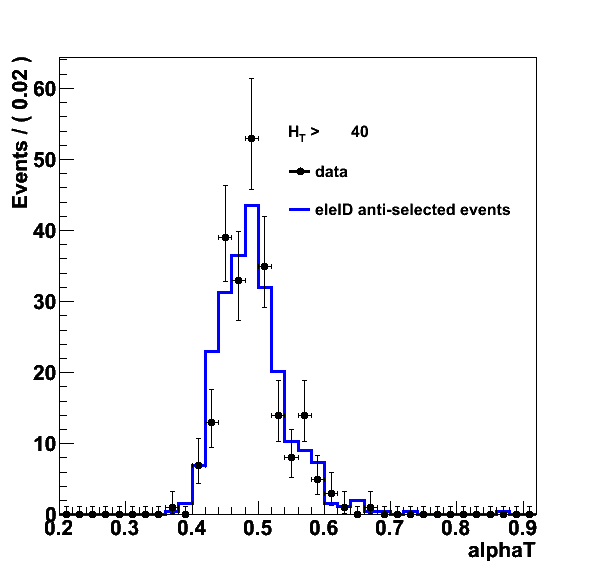
\includegraphics[width=50mm]{Plots/d-alphaT-1}
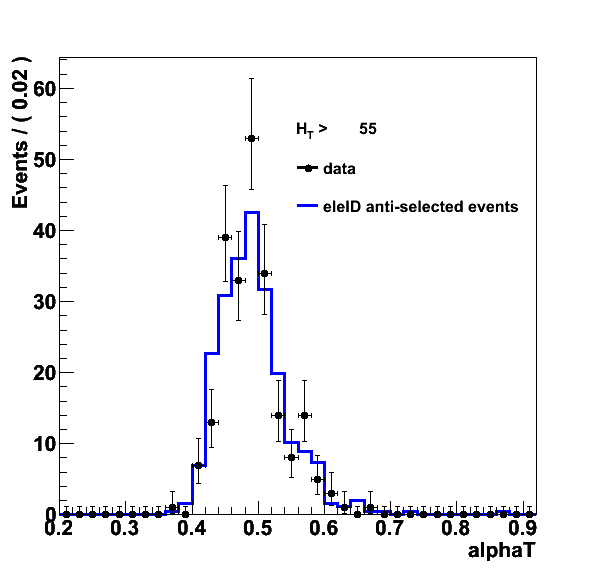
\includegraphics[width=50mm]{Plots/d-alphaT-2}
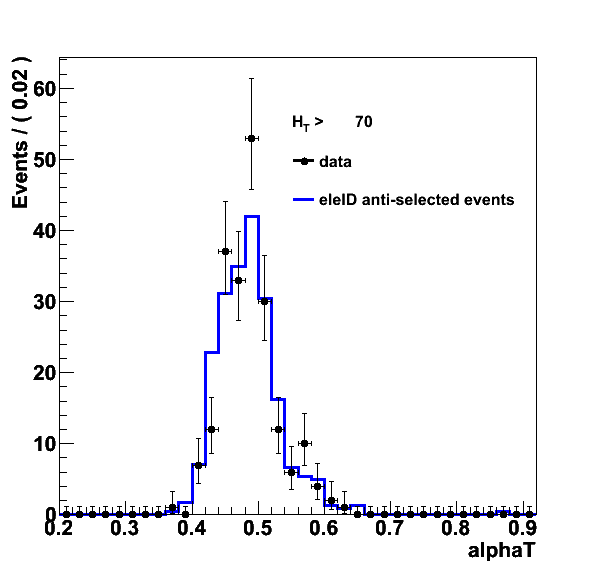
\includegraphics[width=50mm]{Plots/d-alphaT-3}
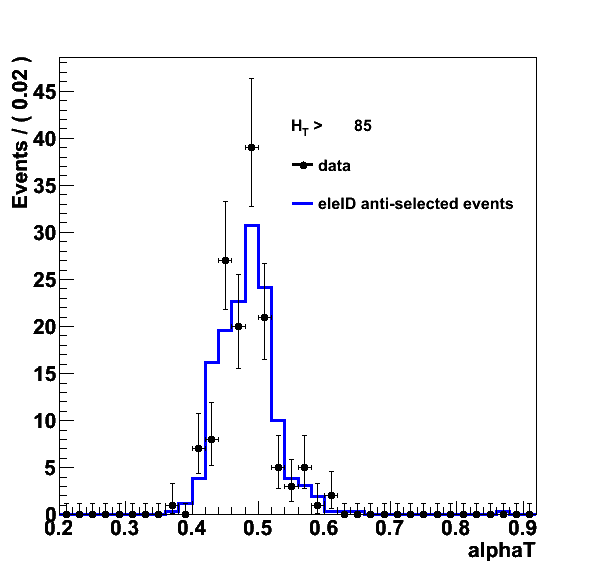
\includegraphics[width=50mm]{Plots/d-alphaT-4}
\hspace*{3mm}
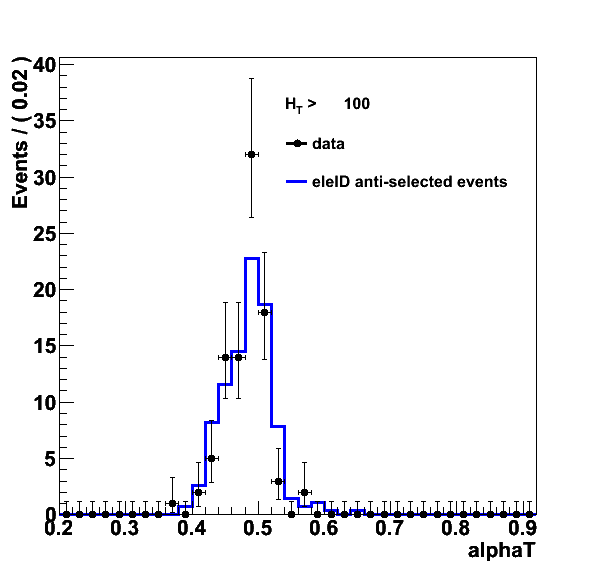
\includegraphics[width=50mm]{Plots/d-alphaT-5}
\hspace*{3mm}
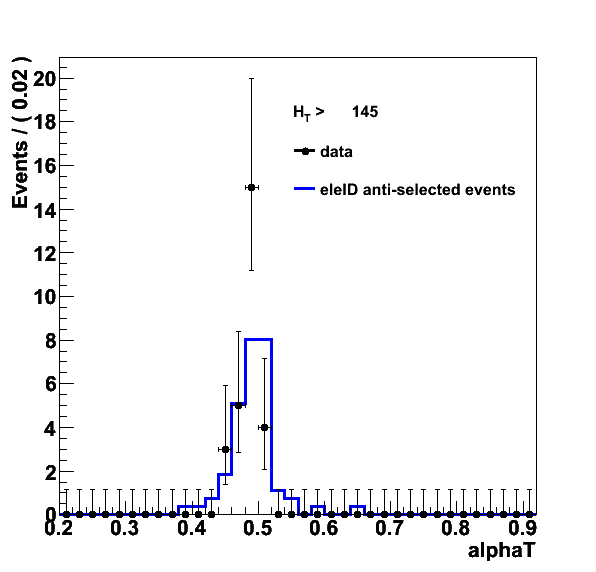
\includegraphics[width=50mm]{Plots/d-alphaT-6}
\caption{\textit{The $\alpha_{T}$ distributions for selected (red) and anti-selected events (black) from collision data shown with progressive cuts in $H_{T}$. These distributions are normalised to each other for shape comparison. There is good agreement between the selected and anti-selected samples regardless of $H_{T}$ requirement, and the high $\alpha_{T}$ tails are reduced as expected when moving to higher $H_{T}$ cuts.}}
\label{fig:datamc}
\end{figure}
%\hspace*{3mm}
\begin{figure}[h!]
\centering
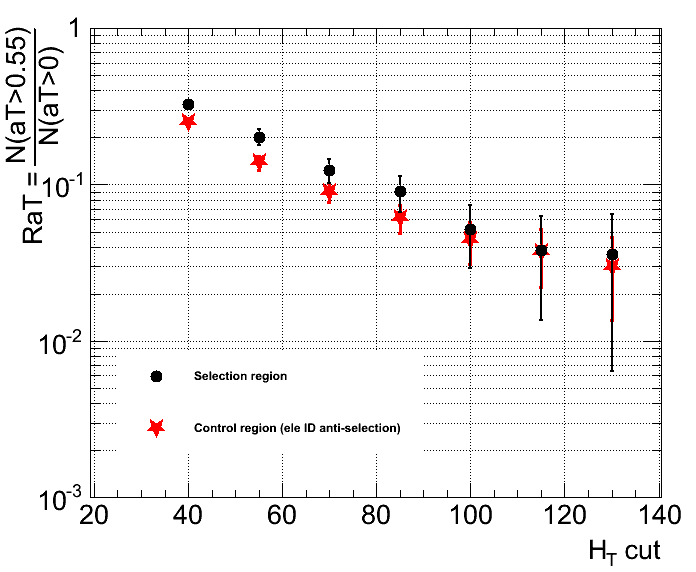
\includegraphics[scale=0.32]{Plots/RaT_pt10.png}
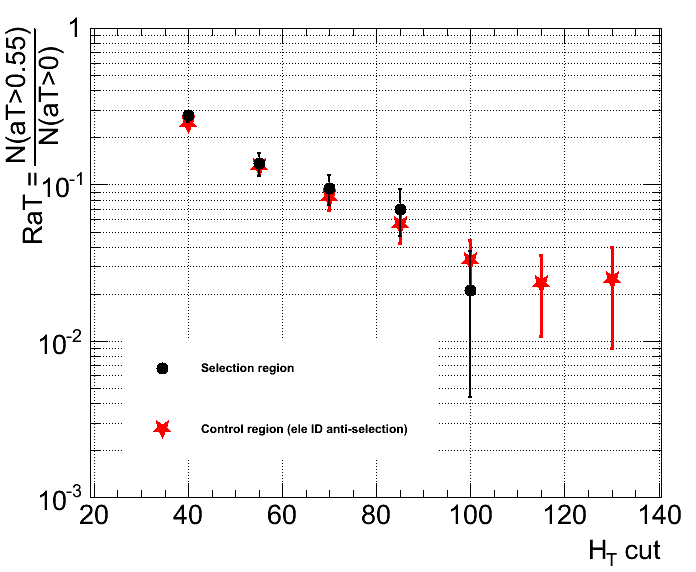
\includegraphics[scale=0.32]{Plots/RaT_pt10_anticut.png}
%\hspace*{13mm}
%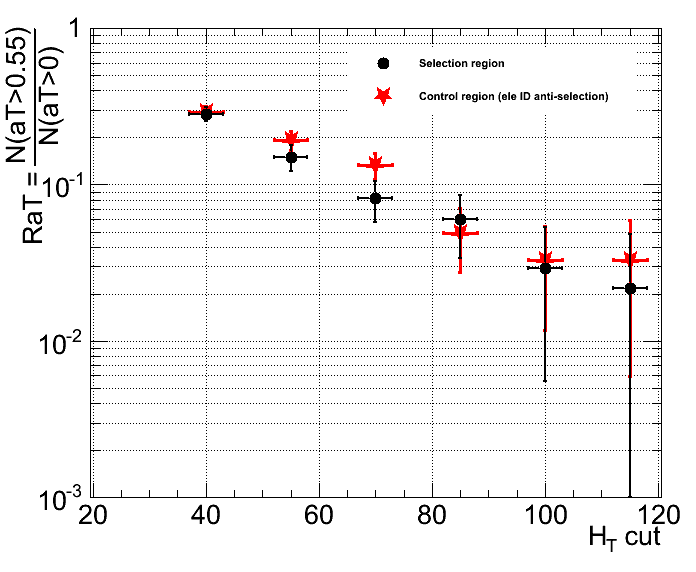
\includegraphics[width=80mm]{Plots/RaT_pt10_anticut_MCP8.png}
\caption{\textit{The $R_{\alpha_T}$ versus the $H_{T}$ cut applied for collision data, shown for both selected and anti-selected events in the ID Inversion method. The right plot includes a cut at pfMET$<20$~GeV to eliminate contamination of prompt electron sources (e.g. Ws). The collision data amounts to 12.47 nb$^{-1}$.}}
\label{fig:datamcRat}
\end{figure}
